\documentclass[border=8pt]{standalone}
\usepackage{fontspec}
\setmainfont{TeX Gyre Heros}[Ligatures=TeXOff]
\XeTeXgenerateactualtext=1
\setsansfont{TeX Gyre Heros}
\usepackage{tikz}
\usetikzlibrary{arrows.meta,positioning,shapes.geometric,shapes.misc,shapes.symbols,fit,backgrounds,calc,chains}
\definecolor{ink}{HTML}{111827}
\definecolor{band}{HTML}{F3F4F6}
\definecolor{band2}{HTML}{E5E7EB}
\definecolor{accent}{HTML}{1D4ED8}
\definecolor{accentlight}{HTML}{DBEAFE}
\definecolor{warn}{HTML}{B91C1C}
\definecolor{warnlight}{HTML}{FEE2E2}
\definecolor{ok}{HTML}{047857}
\definecolor{oklight}{HTML}{D1FAE5}
\tikzset{
  >={Stealth[length=2.6mm]},
  box/.style={draw=ink, line width=0.6pt, rounded corners=9pt, fill=white, align=center,
              inner sep=4pt, font=\small},
  pill/.style={box, rounded corners=13pt},
  key/.style={box, fill=accentlight, draw=accent, line width=0.9pt},
  soft/.style={box, fill=band},
  dec/.style={draw=ink, line width=0.6pt, diamond, aspect=2.2, align=center, inner sep=1.5pt,
              font=\footnotesize, fill=white},
  arr/.style={->, draw=ink, line width=0.6pt},
  darr/.style={->, draw=ink, line width=0.6pt, dashed},
  lbl/.style={font=\footnotesize, fill=white, inner sep=1.5pt},
  layer/.style={draw=band2, fill=band, rounded corners=6pt},
  title/.style={font=\bfseries\small, align=left, anchor=west},
}
\begin{document}
\sffamily\hyphenpenalty=10000\exhyphenpenalty=10000

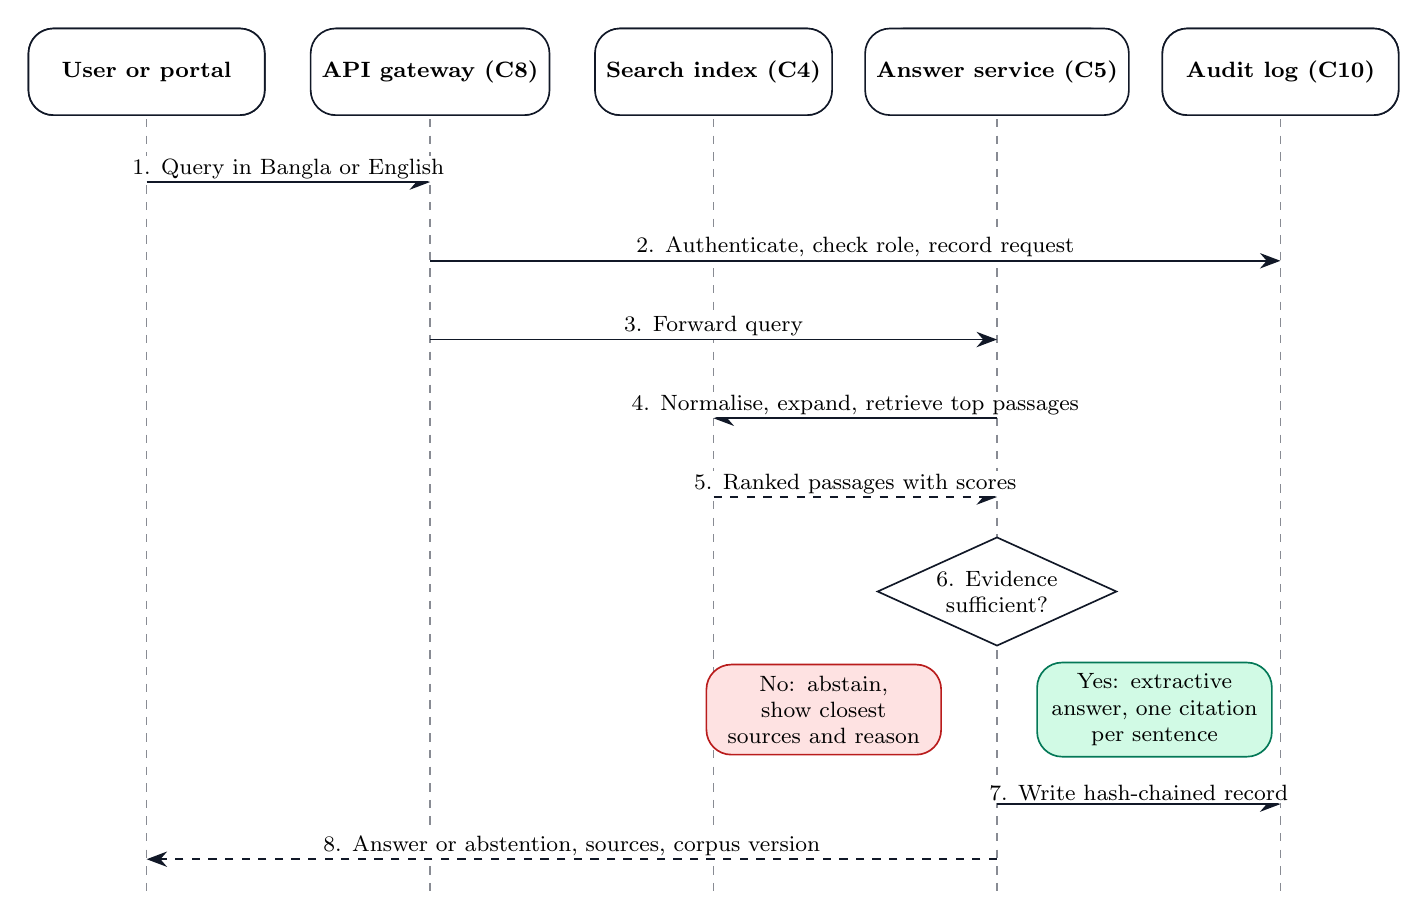
\begin{tikzpicture}
\tikzset{life/.style={box, minimum width=30mm, minimum height=11mm, font=\footnotesize\bfseries},
         msg/.style={->, draw=ink, line width=0.6pt}, ret/.style={->, draw=ink, line width=0.6pt, dashed},
         ml/.style={font=\footnotesize, fill=white, inner sep=1pt}}
\foreach \i/\x/\k in {1/0/u,2/36/g,3/72/s,4/108/a,5/144/l} {
  \node[life] (h\i) at (\x mm,0) {};
  \draw[ink!50, line width=0.5pt, dashed] (\x mm,-6mm) -- (\x mm,-104mm);
}
\node[life] at (h1) {User or portal}; \node[life] at (h2) {API gateway (C8)}; \node[life] at (h3) {Search index (C4)};
\node[life] at (h4) {Answer service (C5)}; \node[life] at (h5) {Audit log (C10)};
\draw[msg] (0,-14mm) -- node[ml, above]{1. Query in Bangla or English} (36mm,-14mm);
\draw[msg] (36mm,-24mm) -- node[ml, above]{2. Authenticate, check role, record request} (144mm,-24mm);
\draw[msg] (36mm,-34mm) -- node[ml, above]{3. Forward query} (108mm,-34mm);
\draw[msg] (108mm,-44mm) -- node[ml, above]{4. Normalise, expand, retrieve top passages} (72mm,-44mm);
\draw[ret] (72mm,-54mm) -- node[ml, above]{5. Ranked passages with scores} (108mm,-54mm);
\node[dec, minimum width=30mm] (ev) at (108mm,-66mm) {6. Evidence\\sufficient?};
\node[box, fill=oklight, draw=ok, font=\footnotesize, text width=27mm] at (128mm,-81mm) {Yes: extractive answer, one citation per sentence};
\node[box, fill=warnlight, draw=warn, font=\footnotesize, text width=27mm] at (86mm,-81mm) {No: abstain, show closest sources and reason};
\draw[msg] (108mm,-93mm) -- node[ml, above]{7. Write hash-chained record} (144mm,-93mm);
\draw[ret] (108mm,-100mm) -- node[ml, above, pos=0.5]{8. Answer or abstention, sources, corpus version} (0,-100mm);
\end{tikzpicture}
\end{document}
